% Created 2021-09-27 Mon 11:52
% Intended LaTeX compiler: xelatex
\documentclass[letterpaper]{article}
\usepackage{graphicx}
\usepackage{grffile}
\usepackage{longtable}
\usepackage{wrapfig}
\usepackage{rotating}
\usepackage[normalem]{ulem}
\usepackage{amsmath}
\usepackage{textcomp}
\usepackage{amssymb}
\usepackage{capt-of}
\usepackage{hyperref}
\doublespacing
\setlength{\parindent}{0pt}
\usepackage[margin=1in]{geometry}
\usepackage{fontspec}
\usepackage{svg}
\usepackage{cancel}
\usepackage{indentfirst}
\setmainfont[ItalicFont = LiberationSans-Italic, BoldFont = LiberationSans-Bold, BoldItalicFont = LiberationSans-BoldItalic]{LiberationSans}
\newfontfamily\NHLight[ItalicFont = LiberationSansNarrow-Italic, BoldFont       = LiberationSansNarrow-Bold, BoldItalicFont = LiberationSansNarrow-BoldItalic]{LiberationSansNarrow}
\newcommand\textrmlf[1]{{\NHLight#1}}
\newcommand\textitlf[1]{{\NHLight\itshape#1}}
\let\textbflf\textrm
\newcommand\textulf[1]{{\NHLight\bfseries#1}}
\newcommand\textuitlf[1]{{\NHLight\bfseries\itshape#1}}
\usepackage{fancyhdr}
\pagestyle{fancy}
\usepackage{titlesec}
\usepackage{titling}
\makeatletter
\lhead{\textbf{\@title}}
\makeatother
\rhead{\textrmlf{Compiled} \today}
\lfoot{\theauthor\ \textbullet \ \textbf{2021-2022}}
\cfoot{}
\rfoot{\textrmlf{Page} \thepage}
\renewcommand{\tableofcontents}{}
\titleformat{\section} {\Large} {\textrmlf{\thesection} {|}} {0.3em} {\textbf}
\titleformat{\subsection} {\large} {\textrmlf{\thesubsection} {|}} {0.2em} {\textbf}
\titleformat{\subsubsection} {\large} {\textrmlf{\thesubsubsection} {|}} {0.1em} {\textbf}
\setlength{\parskip}{0.45em}
\renewcommand\maketitle{}
\author{Albert Huang}
\date{April 9, 2021}
\title{Causes of World War I Essay}
\hypersetup{
 pdfauthor={Albert Huang},
 pdftitle={Causes of World War I Essay},
 pdfkeywords={},
 pdfsubject={},
 pdfcreator={Emacs 28.0.50 (Org mode 9.4.4)}, 
 pdflang={English}}
\begin{document}

\tableofcontents

\setlength\parindent{0.5in}

\section{The Inevitable Shift: How International Incentives Cause Individual Radicals}
\label{sec:orgdc19ba9}

At the turn of the twentieth century, Europe was locked in an arms race caused by level three international political and economic incentives. As tensions grew, level one cultural strifes inevitably intensified and ultimately sparked war.
The plethora of psychological factors that influence individual decisions can be aggregated along various spectra; one such dimension captures how extremely individuals identify with culture over nationality. Charts depicting the distribution of viewpoints provide a multifaceted description of societal status.
Generally, although a lack of enforcement of international order and ballooning militaries both incentivized and enabled WWI, the necessary spark was provided by individual civilian interests.

Reinforcing international incentives such as the security dilemma and cult of the offensive put the international powers on edge, bringing the European powers closer to war.
As a united Germany industrialized, both its population and industrial might grew to rival the French and British powers of the time. For instance, in 1880—nine years after Germany was officially unified—the German empire produced only 8.5\% of the world's manufacturing output while Britain produced 22.9\% of it. By 1913, deep into the security dilemma and one year before the war, Germany had surpassed British production and nearly doubled that of France's (Kennedy Table 18).
Countries tend to grow their military as they industrialize, even if only for defensive purposes. As Germany doubled its military population over three decades to challenge century-long British and French domination, it posed a threat to its neighbors: France and Russia. France and Russia allied with Britain in 1904 and 1907 respectively, which shows their fear of a coming war. These states acted on this mutual fear by increasing militarization, creating a self-reinforcing cycle.
This trend can be generalized as the so-called ``security dilemma," which doubled the number of military and naval personnel worldwide in the 30 years between the German unification and the war, and nearly tripled the global warship tonnage (Kennedy Tables 19-20). A level two perspective would explain this aggression with Germany's expansionist ideals, but even Britain's liberal parliamentary democracy quadrupled its naval tonnage.
Leaders at the time believed that preempting war would allow a fast and decisive victory (Palmer 666). Even simplifying the outcomes to two countries and four possibilities, where each country either attacks or defends, rational actors will choose to preempt war. As a result, each country prepared to invade its neighbors, and tensions grew.

  As a side effect of this global militarization, the populous glorified and anticipated war. This level three influence on the level one psyche inflamed nationalist ideals across Europe and primed a newly-ticking explosive.
  Popular works from the years leading up to the war describe how natural and necessary war is.
  For instance, German general and influential military writer Friedrich von Bernhardi (1849-1930) wrote in the ``immensely popular" (Perry 292) \emph{Germany and the Next War} (1911) that ``War is a biological necessity of the first importance," and that ``every attempt to exclude it from international relations must be demonstrably untenable" (von Benhardi).
  As both a high-ranking general and a best-selling author, von Bernhardi was in a unique position to influence public opinion about warfare. His aggressive stance is not surprising given his military background, and his work was instrumental in priming Germany for battle: a nation cannot go to war without first fostering the support of the populous, as the citizens at large provide the troops, taxes, and labor to sustain warfare. Be it propaganda or national pride, such vehement arguments swayed public opinion and opened the possibility of large-scale battle.
  A level two viewpoint may counter that Germany was naturally expansionist, but similar widespread sentiment in France suggests government structure and ideology were not a sufficient influence on public opinion. French writer Ronald Dorgeles (1885-1973) recalls the mood in Paris at the outbreak of war, writing ``Suddenly a heroic wind lifted their heads. What? War, was it? Well then, let's go!" (Dorgeles).
  The French parliamentary constitutional government had been weakened by civil unrest and was thus incapable of forcing an uncooperative populous to war. However, even the traditionally pacifist left-wing activists agreed in August of 1914 to refrain from calling strikes during the duration of the war in the Union Sacrée or Sacred Union (DBPedia). Thus, French actions could not have been a primarily governmental influence, and such countries went to war due to level three influences on public opinion.
An exclusively level one viewpoint may counter that German writers like Heinrich von Treitschke had been espousing and glorifying war decades before the rapid German industrialization beginning in 1970. However, the shift was more recent in other countries. Dorgeles notes the ideological reversal that socialist workers follow upon hearing of war: ``Seeing their old dreams of peace crumble, [socialist workers] would stream out into the boulevards \ldots{} [but] they would cry 'To Berlin!,' not 'Down with war!'" (Dorgeles). Although Germany's actions may be a result of its level two structure, the level three influence on level one psyche is required to explain the actions of other states.

As countries militarized and nationalist views grew, ethnic and religious divisions intensified until something inevitably sparked war.
  Distributions along these psychological axes can provide a multifaceted snapshot of a societal psyche. A steeper and narrower curve indicates general consensus amongst a population, while a far-flung offshoot indicates a population of extremists. Two peaks is a sign of political polarization, and narrower or more distant peaks are more exetremely polarized.
No matter the axis and the shape of the distribution, the level three influences shifted the general psyche to become more warlike, pushing a few individuals near the extreme end of the ideological bell curve past a critical point. In the case of WWI, the population that crossed the line first was the Yugoslavic population of Austria-Hungary.

\begin{center}
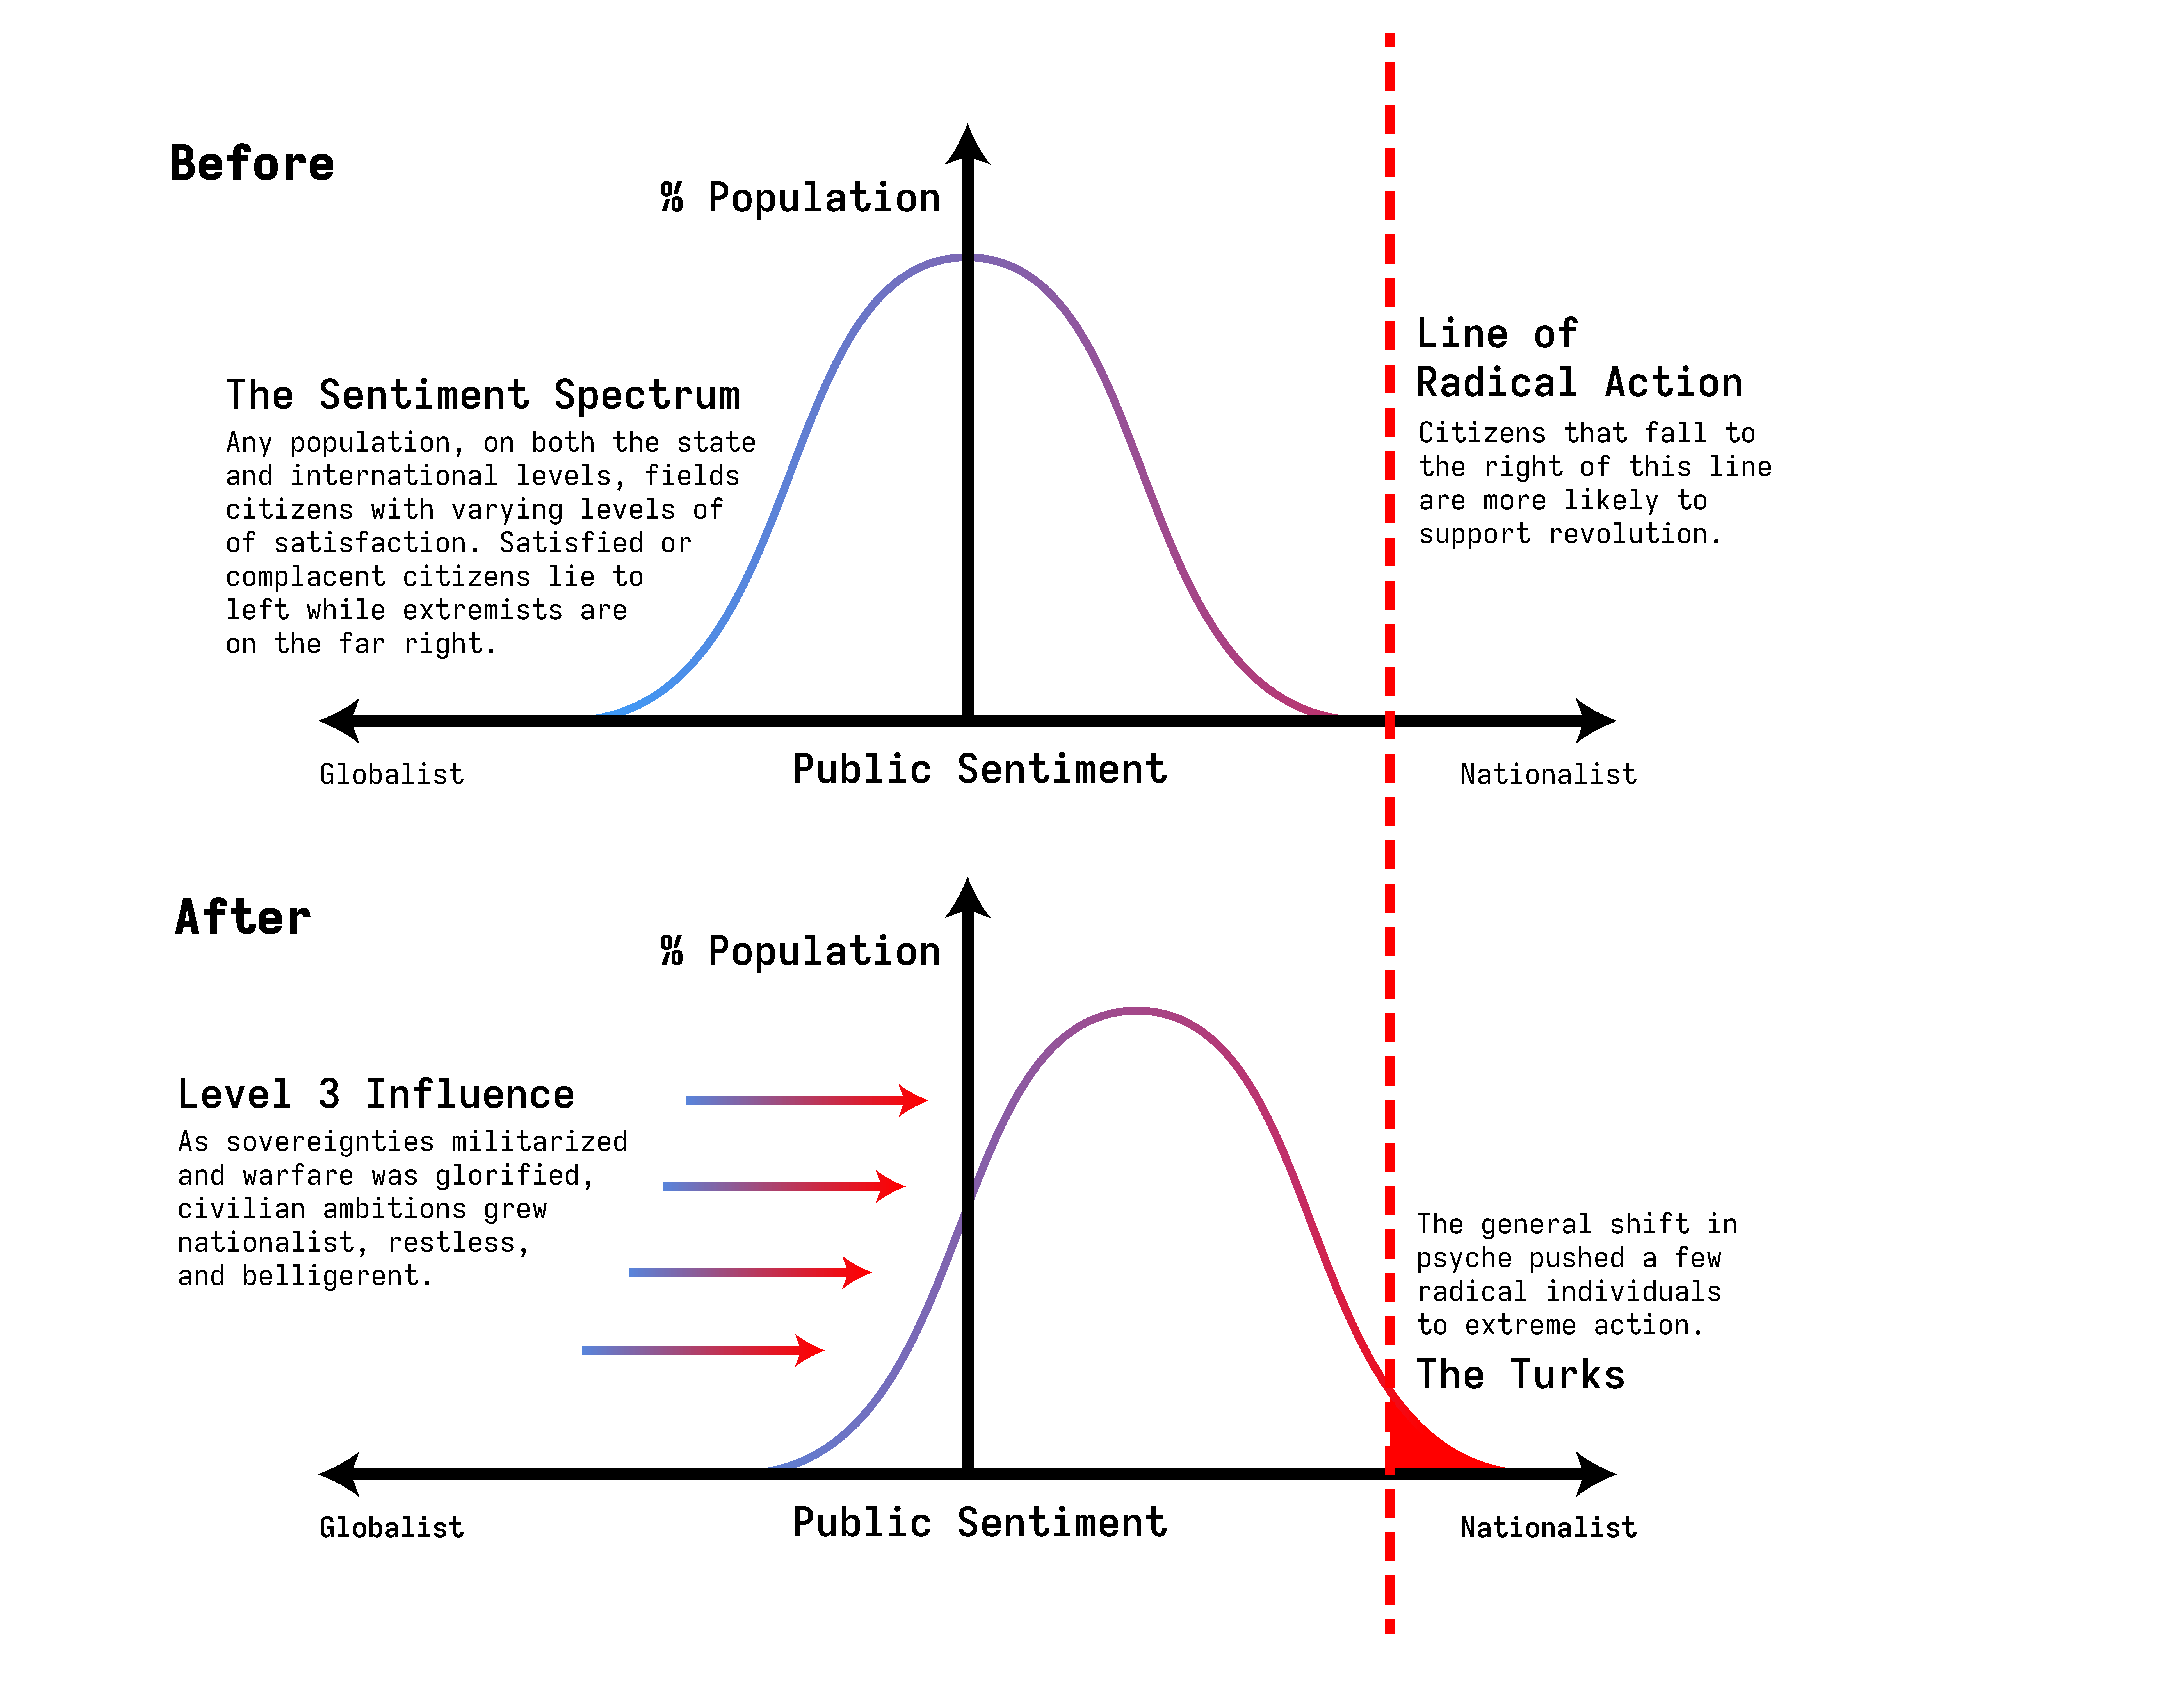
\includegraphics[width=.9\linewidth]{KBe21hist201retCausesOfWWIEssayDiagram.png}
\end{center}

In the case of WWI, the weakest link was the religious divide in Austria-Hungary. Over the course of numerous ``Balkan crises," the Eastern Orthodox Serbs and Bosnians in southern Austria-Hungary grew discontent with the Roman Catholic Dual Monarchy that ruled the Habsburg empire—soon to be Austria-Hungary. As the Ottoman Empire declined, the Serbs marked Bosnia as their own and were infuriated when Austria annexed Bosnia in 1908. When the Balkan wars saw Austria cut Serbia off from the sea, Serbs both independent and Austrian grew exasperated and desperate (Palmer 662).
This chain of events was driven by the recent level three influences—the ongoing security-dilemma-induced arms race had Germany's neighbors scrambling for land and power. States and citizens alike were expecting war, and looking to gain as much of an upper hand as possible before it broke out.
This chain of battles in the Balkans led to increasingly inflamed Serbian nationalism, and the breaking point came on the 28th of June, 1914 when Bosnian Serb Gavrilo Princip assassinated Archduke Franz Ferdinand of Austria and sparked the Great War.

As power dynamics shifted around the turn of the twentieth century, the defined scarcity of state goals---such as the British ambition of having the largest navy---set off a chain of events that ultimately led to the inevitable global war. Without a change of level three incentives, such as a global mediator or mutually assured destruction, shifting power dynamics and the cult of the offensive will lead, and did lead, inescapably to a security-dilemma-induced arms race and growing tensions which cause nationalist viewpoints and inspire rash individuals. Thus, international disincentives like mutually assured destruction are key to keeping political and economic incentives from inflaming ideological divides and causing warfare.

\section{Works Cited}
\label{sec:org34e8eaa}

\begin{itemize}
\item Kennedy, Paul M. \emph{The Rise and Fall of the Great Powers: Economic Change and Military Conflict from 1500 to 2000}. 1987. Print.
\item Perry, Jonathan S. \emph{Sources for Europe in the Modern World}. Oxford University Press, 2016.
\item ``About: Sacred Union." DBPedia, dbpedia.org/page/Sacred\_ Union. Accessed 7 Apr. 2021.
\item Palmer et al. \emph{A History of the Modern World}, 9th Edition.
\item Urban, Tim. “The Enlightenment Kids.” \emph{Wait But Why}, 3 Oct. 2020, waitbutwhy.com/2019/09/enlightenment-kids.html. Sentiment distribution chart loosely inspired by this blog post.
\end{itemize}
\end{document}
